\chapter{Metodologia}\label{ch:work}
\section{JPEG AI Verification Model}\label{sec:vm}
%tipi dei dati, struttura, target bpp e altri parametri.
Lo strumento utilizzato per ottenere la codifica JPEG AI è "jpeg-ai-reference-software" \cite{jpeg-ai-ref-sw} che rappresenta il software di riferimento per la prima implementazione del sistema proposto chiamato \textit{JPEG AI Verification Model} \cite{wg1n100279}. Sono proposti due encoder con diversi livelli di complessità: \texttt{Enc0}, il più semplice, progettato per dispositivi mobili, ed \texttt{Enc1}, più complesso, composto da \textit{attention blocks} e\textit{ transformer}, necessitando quindi capacità computazionale elevata.
Sono supportati tre diversi "operation point" SOP (\textit{Simple Operation Point}), BOP (\textit{Basic Operation Point}) e HOP (\textit{High Operation Point}) ottimizzati rispettivamente per l'uso su dispositivi dotati di CPU, dispositivi mobili, e dispositivi dotati di hardware specializzato come le GPU.
\begin{figure}
    \centering
    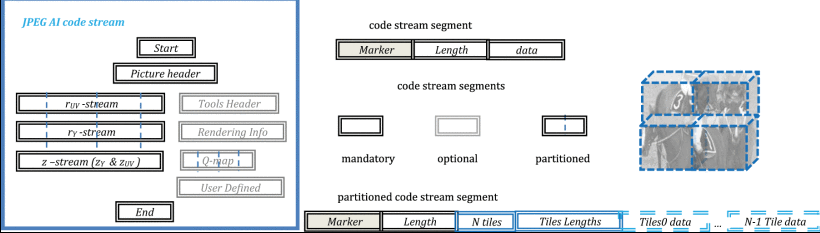
\includegraphics[width=1\linewidth]{img/JPEG AI codestream.png}
    \caption{JPEG AI bitstream}
    \label{fig:bitstream}
\end{figure}
% PARLARE DI VARIABILE RATE O BRM?
\section{Dataset utilizzato}\label{sec:dataset}
Il dataset usato negli esperimenti è \textit{140k Real and Fake Faces} \cite{140kRealFake}, una raccolta di 140.000 immagini di volti, suddivise in 70.000  immagini reali e 70.000 immagini fake.
I dati sono già suddivisi in training set, test set, e validation set, rispettivamente composti da 100.000, 20.000 e 20.000 immagini; ogni insieme mantiene un perfetto bilanciamento tra le due classi; queste caratteristiche rendono il dataset ideale per l'addestramento semplificando la preprarazione dei dati. Le immagini sono in formato JPEG e sono state ridimensionate in 256x256 pixel; sono inclusi file csv contententi le etichette e il percorso di ogni immagine.
\paragraph{Immagini reali}Le immagini reali fanno parte del dataset \textit{Flickr-Faces-HQ} (FFHQ) \cite{NVlabsFfhqdataset2025}, il dataset creato per lo sviluppo di StyleGAN, e consistono in fotografie di volti umani di alta qualità (risoluzione a 1024x1024). Questo si distingue da altri dataset per la presenza di una grande varietà di soggetti per età ed etnia, ma anche per la presenza di accessori come occhiali o cappelli \cite{karras2019style} rendendolo molto diversificato; queste immagini sono state collezionate da Flickr, un servizio web che offre la possibilità di pubblicare immagini ad artisti e fotografi.
\paragraph{Immagini sintetiche}Le immagini fake invece fanno parte del dataset \textit{1 Milion Fake Faces} ,un insieme di immagini generate tramite StyleGAN (vedi sez. \ref{par:style}). 
\section{Classificatori utilizzati}
Sono stati scelti due diversi algoritmi di classificazione, Random Forest e GradientBoosting, entrambi appartenenti alla categoria degli \textit{ensemble methods}. Questa classe di algoritmi si basa sull'idea di combinare le predizioni di più modelli base detti 'deboli' (\textit{weak learners}) per creare un modello finale con maggior accuratezza.
\subsection{Random Forest}
Random Forest è un algoritmo di apprendimento supervisionato che utilizza alberi di decisione come modelli deboli.\\
Gli alberi di decisione fanno predizioni attraverso una serie di test sugli attributi dei dati. La costruzione di un albero di decisione si basa sul concetto di ripartizione ricorsiva dello spazio di input in sottinsiemi di dimensione minore, scegliendo l'attributo da testare in base al guadagno informativo derivato da quella scelta, cercando di minimizzare l'impurità dei sottoinsiemi.
%Misure di purezza
L'aspetto critico di questa tecnica è l'alta varianza, infatti cambiamenti nei dati di addestramento influenzano molto la struttura dell'albero finale.

Questo problema può essere risolto con l'uso della tecnica di \textit{bagging} ((Bootstrap Aggregating)) che consiste nel creare $K$ diversi sottoinsiemi campionando con reinserimento (\textit{Bootstrap}) dall'insieme di addestramento originale ed allenare su ogni sottoinsieme un modello base. La predizione finale viene fatta aggregando (\textit{Aggregating}) le predizioni dei $K$ modelli. Questo permette una riduzione della varianza, ma presenta il problema di forte correlazione dei modelli base che vengono creati, sopratutto quando un attributo risulta avere un guadagno informativo più alto, diventando radice per molti alberi.\\
Nei Random Forest questo problema viene risolto variando  l'insieme di attributi tra cui poter scegliere quello sul quale fare il test, garantendo una bassa correlazione tra gli alberi.
\subsection{Gradient Boosting}
La differenza principale dell'algoritmo di Gradient Boosting rispetto a Random Forest risiede nell'uso del \textit{boosting}.
Nel boosting ogni dato di esempio ha un peso che indica la sua importanza nell'addestramento. L'idea è quella di allenare un insieme di modelli deboli in modo sequenziale: partendo con un insieme con lo stesso peso per tutti gli esempi viene addestrato il primo modello. Prima di allenare il modello successivo, i pesi vengono aggiornati facendo sì che il peso degli esempi classificati in modo errato venga incrementato, mentre quello degli esempi classificati correttamente viene ridotto. Iterando il processo per $K$ iterazioni vengono prodotti $K$ modelli deboli tra i quali almeno un modello riuscirà a classificare in modo corretto anche gli esempi più difficili.\\
Per fare la predizione, ogni modello debole vota, e la predizione finale viene fatta considerando il voto di maggioranza.\\
Nel Gradient Boosting, il processo di boosting non si basa sui pesi, ma sul gradiente negativo della funzione di perdita: partendo con una funzione di perdita differenziabile, si fanno le predizioni e si calcola per ogni esempio il gradiente negativo della funzione di perdita. Con questa informazione viene addestrato un nuovo modello debole aggiornando i parametri muovendosi nella direzione del gradiente negativo. 
\subsection{Hyperparameter Tuning}\label{subsec:tuning}
Le prestazioni dei modelli di apprendimento spesso dipendono dalla scelta degli iperparametri. Questi sono i parametri di configurazione del modello che non vengono appresi automaticamente. È buona pratica adottare la tecnica di \textit{hyperparameter tuning} per trovare la combinazione di iperparametri che offre migliori prestazioni.
La ricerca viene fatta scegliendo modello e lo spazio dei valori degli iperparametri da esplorare, e si possono adottare diverse tecniche.\\
La ricerca a griglia (\textit{Grid Search}) compie una ricerca esaustiva sulla griglia degli iperparametri specificati, generando un modello per ogni combinazione possibile. Questa, anche se molto onerosa dal punto di vista computazionale, garantisce di trovare la combinazione ottimale tra quelle specificate.\\
La ricerca casuale (\textit{Random Search}) invece effettua un campionamento di un numero finito di valori dei parametri seguendo una distribuzione scelta. Questa tecnica risulta molto più efficiente rispetto alla ricerca a griglia, riuscendo comunque a trovare buone combinazioni di iperparametri; viene usata principalmente quando lo spazio di ricerca ha alta dimensionalità.\\
La valutazione delle prestazioni dei modelli viene utilizzata la \textit{k-fold cross-validation}, un'operazione che suddivide l'insieme di addestramento in $k$ sottoinsiemi, e addestra il modello su k-1 sottoinsiemi per poi testarlo su quello rimanente; il modello scelto sarà quello che ha ottenuto una migliore accuratezza.
\section{Pipeline degli esperimenti}\label{sec:pipeline}
\subsection{Rappresentazioni latenti estratte da JPEG AI}\label{subsec:latenti}
Le immagini prima di essere elaborate dall'encoder vengono convertite nello spazio di colori YUV BT.709, separando le componenti di luminanza e crominanza. Successivamente viene applicata la CCS (\textit{Conditional Color Separation}) \cite{10018070}, una tecnica con cui la componente primaria, la luminanza ($Y$), viene compressa con una rete neurale più complessa e potente, per preservare più informazioni possibili, mentre per le componenti di crominanza ($UV$) la compressione avviene sfruttando informazioni della luminanza.
La separazione delle componenti è mantenuta anche nel bitstream finale (vedi fig. \ref{fig:bitstream}) dando la possibilità di scartare la parte di crominanza se non necessaria per l'applicazione scelta.\\
Nel processo di codifica JPEG AI genera un dizionario contenente tutti i valori necessari utilizzati nel resto dell'architettura (vedi fig. \ref{fig:architmin}). Per l'obbiettivo di questo lavoro i classificatori utilizzeranno y e y\_hat che rappresentano rispettivamente l'output dell'\textit{Analysis transform} ($y$ vedi fig.\ref{fig:encodingJPEGAI}) , e l'input dell'\textit{Synthesis transform} ($\hat{y}$ vedi fig. \ref{fig:decodingJPEGAI}), ovvero la versione di y quantizzata. Entrambi sono composti da tensori nominati \texttt{model-y} e \texttt{model-uv} per rappresentare componenti di luminanza e crominanza separatamente, come voluto dal meccanismo di CCS. Questi tensori hanno rispettivamente dimensione (160, 16,16) e (96, 16, 16).\\
\subsection{Preprocessing dei latenti}\label{sec:preprocessing}
Per allenare i modelli di classificazione scelti è necessario trasformare i tensori prodotti dall'encoder in vettori unidimensionali; sono state utilizzate diverse strategie applicabili alla sola componente di luminanza, oppure a tutte le componenti YUV, caso in cui tutti i vettori ottenuti vengono concatenati.
\paragraph{Flattening} La prima strategia testata è stata più semplice ed intuitiva da realizzare, trattandosi di un'operazione di \textit{flattening}: il tensore multidimensionale viene trasformato in un vettore concatenando tutti i valori presenti.\\
\paragraph{Estrazione di patch} La seconda strategia adottata consiste nell'estrazione di patch dal tensore, dove ogni patch è il risultato della concatenazione dei valori presenti nelle stesse posizioni spaziali per tutti i canali dei tensori. In questo modo si ottiene un vettore di dimensione inferiore rispetto all'uso della tecnica di flattening, rendendo l'addestramento più rapido e meno dispendioso in termini di memoria.\\
Di questa tecnica sono state utilizzate due varianti: \textit{Single Patch}, nella quale per ogni tensore viene estratta una singola patch (quella centrale), e \textit{N Patches}, dove invece vengono estratte N patch in posizioni. In questo secondo caso, ogni patch viene considerata come un esempio indipendente, aumentando la cardinalità dell'insieme di addestramento.
\\

La scelta del metodo di preprocessing delle feature influenza la struttura del dataset e le modalità di valutazione del modello. Nella tabella \ref{tab:preprocessing_methods} viene proposta una schematizzazione dei metodi.
\begin{table}[H]
\centering
\caption{Confronto tra metodi di preprocessing delle feature.}\label{tab:preprocessing_methods}
\begin{tabularx}{\textwidth}{l c c}
\toprule
\textbf{Method} & \textbf{Samples per Image} & \textbf{Feature Dimension} \\
\midrule
Flatten Latents (Y)        & 1 & $C_y \cdot H \cdot W = 40960$ \\
Flatten Latents (YUV)     & 1 & $(C_y +C_{uv})\cdot H \cdot W = 65536$ \\
Single Patch (Y)        & 1 & $C_y = 160$ \\
Single Patch (YUV)     & 1 & $C_y + C_{uv} = 256$ \\
N Patches (Y)    & N & $C_y = 160$ \\
N Patches (YUV)        & N & $C_y + C_{uv} = 256$ \\
\bottomrule
\end{tabularx}
\small{Nota: $H,W$ sono le dimensioni di ogni canale dei tensori, $C_y, C_{uv}$ sono il numero di canali rispettivamente della componente Y e delle componenti U e V.}
\end{table}
Per il metodo N Patches, la fase di testing viene svolta in maniera differente rispetto alle altre: nella fase di addestramento, per ogni immagine vengono estratte N patches ottenendo un insieme di addestramento di cardinalità $N\cdot |\mathcal{D}|$ (dove $\mathcal{D}$ è il dataset originale). Per la fase di testing invece si utilizza la strategia di \textit{majority voting}: per ogni immagine vengono estratte tutte le patch, ed il classificatore produce una predizione indipendente su ognuna di queste. La predizione finale sarà la classe più frequente tra tutte le votazioni.
\subsection{Esperimenti condotti}\label{sec:experiments}
Come dichiarato nelle sezioni precedenti, l'obbiettivo del lavoro consiste nella verifica dell'efficacia della codifica JPEG AI nel compito di identificazione di immagini sintetiche.\\
Gli esperimenti sono stati condotti per ciascun classificatore scelto analizzando le prestazioni al variare di alcuni fattori principali: livello di compressione (\textit{Bpp}), metodo di preprocessing applicato sulle feature estratte (\textit{Preprocess}), componente scelta e quantizzazione della rappresentazione latente. Nella tabella \ref{tab:experimentalfactors} è riportata una sintesi dei fattori considerati.
\begin{table}[H]
\centering
\caption{Fattori considerati durante gli esperimenti}\label{tab:experimentalfactors}
\begin{tabularx}{\textwidth}{l >{\raggedright\arraybackslash}X}
\toprule
\textbf{Fattore} & \textbf{Valori} \\
\midrule
Livello di compressione (Bpp) & 12bpp, 6bpp \\
\midrule
Componente & Y e YUV \\
\midrule
Preprocessing & Flatten, Single Patch, Multiple Patches \\
\midrule
Versione dei latenti & y (non quantizzato) e y\_hat (quantizzato) (vedi sez. \ref{subsec:latenti})\\
\bottomrule
\end{tabularx}
\end{table}
\subsection{Motivazioni delle scelte}\label{subsec:choices}
La scelta di analizzare le performance a diversi livelli di compressione è motivata dal fatto che questo fattore influisce sulla quantità informativa contenuta nelle rappresentazioni latenti, con una maggior perdita di informazioni a bpp più bassi.\\
L'analisi dell'impatto della componente scelta su cui fare l'addestramento è stata svolta per verificare se l'informazione aggiuntiva presente nella componente di crominanza risulti in un miglioramento nelle prestazioni.\\
Anche con l'uso di diversi metodi di preprocessing si vuol valutare l'impatto dell'informazione disponibile sulla capacità di classificazione. Infatti, come riportato nella tabella \ref{tab:preprocessing_methods}, il metodo di flattening fornisce delle feature con dimensionalità molto elevata rispetto agli altri metodi, e quindi è ragionevole pensare che sarà il migliore tra i risultati.\\
Infine, il confronto delle performance ottenute utilizzando y (non quantizzato) e y\_hat (quantizzato) permette di valutare l'impatto del processo di quantizzazione delle rappresentazioni latenti. Infatti la rappresentazione non quantizzata dovrebbe contenere più informazioni caratterizzanti per la classificazione, e per questo i modelli allenati su questa dovrebbero performare meglio.

\subsection{Fase di addestramento e valutazione dei modelli}\label{subsec:training}
Come descritto nella sez. \ref{subsec:tuning}, per ogni esperimento è stato svolto il tuning degli iperparametri: inizialmente è stata applicata una ricerca casuale su un intervallo di valori ampio e, osservando i risultati ottenuti, è stata svolta una ricerca a griglia ristretta sui 3 migliori valori trovati per ogni iperparametro. I valori trovati da questa prima fase sono stati usati per allenare i modelli finali su $30.000$ immagini, e poi valutarli su $3.000$ immagini di test.

La libreria scelta per gli algoritmi di machine learning è \textit{Scikit-learn}, libreria open-source scritta in Python, che offre strumenti semplici ma efficienti per molte task tra cui quelle di classificazione.
In particolare, per Random Forest è stato utilizzato \texttt{RandomForestClassifier}, mentre per Gradient Boosting \texttt{HistGradientBoostingClassifier}. La libreria scelta mette a disposizione anche algoritmi di ricerca degli iperparametri, tra cui \texttt{RandomizedSearchCV} per la ricerca casuale e \texttt{GridSearchCV} per la ricerca a griglia.
